%=================================================================
\chapter{FLEX Hardware}
\label{ch:hardware}
%=================================================================

%-----------------------------------------------------------------
\section{Architecture}
\label{sec:architecture}
%-----------------------------------------------------------------
The modular architecture provided by FLEX allows to compound a number of boards to integrate different features into a single device.\\

\noindent The basic configuration of a FLEX device is made by the main board only. The FLEX Base Board, refer Figure ~\ref{fig:base}, mounts a Microchip dsPIC� DSC micro-controller, and exports almost all the pins of the micro-controller. To build a specific application, the user can easily connect the desired components to the dsPIC� DSC ports.

\begin{figure}[!ht]
	\centering
		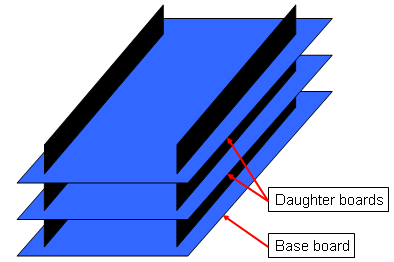
\includegraphics[width=0.65\textwidth, bb=0 0 394 262]{images/piggyback.png}
	\caption{Piggybacking of FLEX Boards}
	\label{fig:piggyback}
\end{figure}

\noindent As depicted in the Figure ~\ref{fig:piggyback}, several Daughter Boards, refer Section ~\ref{sec:daughter}, can be connected in piggyback fashion to the FLEX Base Board, refer Section ~\ref{sec:base}. The Daughter Boards have different features and they can be easily combined to obtain complex devices, refer Section ~\ref{sec:packs}. Evidence Srl and Embedded Solutions supply a growing number of Daughter Boards for basic and advanced applications.\\